\documentclass[12pt,letterpaper]{article}
\usepackage{natbib}

%Packages
\usepackage{xcolor}
\usepackage{color,soul}
\usepackage{pdflscape}
\usepackage{fixltx2e}
\usepackage{textcomp}
\usepackage{fullpage}
\usepackage{float}
\usepackage{latexsym}
\usepackage{url}
\usepackage{epsfig}
\usepackage{graphicx}
\usepackage{amssymb}
\usepackage{amsmath}
\usepackage{bm}
\usepackage{array}
\usepackage[version=3]{mhchem}
\usepackage{ifthen}
\usepackage{caption}
\usepackage{hyperref}
\usepackage{amsthm}
\usepackage{amstext}
\usepackage{enumerate}
\usepackage[osf]{mathpazo}
\usepackage{dcolumn}
\usepackage{lineno}
\usepackage{dcolumn}
\usepackage{hyphenat}
\usepackage[T1]{fontenc}
\usepackage{textcomp}
\newcolumntype{d}[1]{D{.}{.}{#1}}

\pagenumbering{arabic}


%Pagination style and stuff
\linespread{2}
\raggedright
\setlength{\parindent}{0.5in}
\setcounter{secnumdepth}{0} 
\renewcommand{\section}[1]{%
\bigskip
\begin{center}
\begin{Large}
\normalfont\scshape #1
\medskip
\end{Large}
\end{center}}
\renewcommand{\subsection}[1]{%
\bigskip
\begin{center}
\begin{large}
\normalfont\itshape #1
\end{large}
\end{center}}
\renewcommand{\subsubsection}[1]{%
\vspace{2ex}
\noindent
\textit{#1.}---}
\renewcommand{\tableofcontents}{}
%\bibpunct{(}{)}{;}{a}{}{,}

%---------------------------------------------
%
%       START
%
%---------------------------------------------

\begin{document}

%Running head
\begin{flushright}
Version dated: \today
\end{flushright}
\bigskip
\noindent RH: disparate views on disparity.

\bigskip
\medskip
\begin{center}

\noindent{\Large \bf Variations in multidimensional space.} 
\bigskip

\noindent {\normalsize \sc Thomas Guillerme$^{1,*,+}$, Natalie Cooper$^{2,+}$, Stephen Brusatte$^3$, Katie Davis$^4$, Andrew Jackson$^5$, Sylvain Gerber$^6$, Anjali Goswami$^2$, Kevin Healy$^7$, Melanie Hopkins$^8$, Graeme Lloyd$^9$, Joseph O'Reilly$^{10}$, Abi Pate$^{10}$, Emilie Rayfield$^{10}$, Erin Saupe$^{11}$, Emma Sherratt$^{12}$, Graham Slater$^{13}$, Gavin H Thomas$^{14}$ and Philip Donoghue$^{10,+}$}\\


\noindent {\small \it 
$^1$School of Biological Sciences, University of Queensland, St. Lucia, Queensland, Australia.; $^2$NHM; $^{10}$Bristol}
\end{center}
\medskip
\noindent{+ These authors contributed equally to the manuscript.}
\noindent{*\bf Corresponding author.} \textit{guillert@tcd.ie}\\  
\vspace{1in}

%Line numbering
\modulolinenumbers[1]
\linenumbers


%---------------------------------------------
%
%       ABSTRACT
%
%---------------------------------------------

\newpage
\begin{abstract}

\begin{enumerate}
    blablalbalba
\end{enumerate}

\end{abstract}

\noindent (Keywords: disparity)\\

\vspace{1.5in}

\newpage 

%---------------------------------------------
%
%       INTRODUCTION
%
%---------------------------------------------



\section{Introduction}

%1 -
% History of disparity methods
Since the time of the ancient, it has been observed that variation in morphologies often follows discrete patterns rather than a continuous gradient of forms.
These clusters of morphological groups, or, rather their differences (i.e. the disparity of shapes) was popularised in seminal palaeobiology papers in the 1990s [Runnegar 1987, Gould, Foote, Webb, etc.].
Disparity is since then used to describe a particular biological, phenotypic, and/or trait variation without strict distinction between the ontology and epistemology (see Semantic Box).
Over the last 30 years, disparity has been commonly used in the morphological disparity context.
The impressive amount of literature published since then tackles a vast array of biological questions, using different (sometimes contrasted) methods but often consists studies of the phenotype at a macroevolutionary level (i.e. species or above).
To this date, there is no consensus on whether disparity should be restricted and specific to these kind of studies or whether it should be used as a broader umbrella term designating studies of multivariate variation, not restricted in its questions, methods and disciplines.
Throughout this review, we aim to highlight the diversity of disparity analyses and how they can help understanding or provide a structure to biodiversity.
In essence, we suggest that disparity is a pattern of variation.

%2§ what use: commonly used
In evolutionary biology, the description of these patterns has been used to tackle a vast array of questions.
For example, it has been used (1) in Evo-devo to tackle questions of
%evo-devo
Developmental constraints [CITE];
Relationship between form and function and evolution functional traits [CITE] or
Scaling micro to macro [CITE];
% Ecology
(2) in ecology or palaeoecology to study:
intra-specific competition [CITE],
niche occupants, speciation and competition[CITE] or
macroecology (disparity in space)[CITE];
% Evolution
(3) on in macroevolution to study:
response to extinction and selectivity [CITE],
intra-specific competitive replacements [CITE] or
more globally, tempo and mode of evolution [CITE].

%3§ problems
Disparity studies have a great deal of promise in helping us to understand the evolution of biological diversity.
With the expansion of such methodological approaches in the last decade, however, we also identify three main issues that, if not tackled could reduce the power of such analysis.
First, many recent studies have lost focus; they are no longer hypothesis-driven, instead they are undertaken to characterise biological variation for its own sake.
Second, even where there is a clear question being explored, the data being used for disparity analyses is inappropriate and often driven by the availability of large datasets.
Third, the methods being used to analyse these datasets may not always be appropriate for the question and/or data at hand.
Here we deal with some of these issues and present best practice guidelines to allow researchers to optimise their questions before performing a disparity analysis.

\subsubsection{[Box]Disparity patterns or processes}
\label{box_semantic}
At the core of defining what \textit{is} disparity lies a potential divide between epistemology and ontology:
is there a difference between the pattern (and how researchers characterise it) and how it was ultimately generated?
If disparity describes patterns of variation, the underlying scientific question ultimately always needs to use them as a proxy for explaining the biological processes.
In the seminal papers from the late 80s, disparity was solely use to describe and understand the Cambrian Explosion were both the pattern (a high observed dissimilarity between groups) was directly linked to the process (and explosive radiation of multicellular life as championed by Gould).
Restricting disparity to this initial informal definition (multidimensional morphological at a macroevolutionary scale) can be advantageous for advances in this field but broadening it will allow more interdisciplinary discussion.
In fact, in the last years, disparity was also used as a potential tool for investigating ecological processes (disconnected from evolution: e.g. function [CITE], community structure[CITE], competition[CITE]).
In other words disparity could not only inform us on macroevolutionary patterns and processes but also something about environments and ecosystem functioning (with the advantages of easily allowing palaeocological and palaeoenvironemental perspectives).
\subsubsection{[Box]End}

\section{Best practices for disparity analysis}

\section{Find a question}
Why to perform a disparity analysis?
This question might sound like an obvious question to start with but we would like to stress its crucial importance.
The last decade have seen a vast array of excellent methodological implementation and documentations rendering disparity analysis easy to perform \citep{bouxin2005ginkgo,oksanen2007vegan,geiger2008,zelditch2012geometric,adams2013geomorph,Claddis,dispRityv02,adams2017geometric}.
However, this facilitation might (conscientiously or not) pushes authors to perform disparity analysis ``just because'' (i.e. simply because of their facility rather than stemming from a conscious hypothetico-deductive approach).
It is thus important not to rush in a disparity analysis to avoid some basic statistical caveats.
For example, one major thing to consider is circularity: if ones aim is to explore the variation in the data set, a multi-dimensional analysis is perfectly valid.
However, the groups resulting from this exploratory analysis are then no more appropriate for testing a hypothesis [CITE stats 1.0].
Instead, it is more appropriate do the data exploration on a subset of the data (preliminary analysis) and then use the full data set to test the resulting hypothesis.
Clearly framing such hypothesis and their null expectancy will help designing better disparity analysis: which data and methods will be appropriate to test it?

\section{Collect the appropriate data}
If disparity is used to describe patterns for explaining some process, every possible data will always only be a proxy for these patterns.
Tangentially, more data is not necessarily better, especially when the data was originally designed and collected for different questions (e.g. cladistic data - see below).
Therefore, clearly framing the question as indicated above will help avoiding some major caveats.
For example, if a study is focussing on the ecological adaptive radiation of a group, ecological traits must be crucial an might be preferred to purely evolutionary traits.

\subsection{Which type of data}
Morphological disparity analysis can be based on three main types of data:
\begin{enumerate}
    \item discrete data that can be either describing feature (often referred to as ``cladistic''; e.g. the presence or absence of legs, the colour of a tail, etc. [CITE]) or more simply counts (e.g. number of digits, etc. [CITE]);
    \item continuous data that can be either direct measurements (e.g. body length, etc. [CITE]) or more sophisticated methods (e.g. geometric morphometrics, mathematical contour description, etc. [CITE]);
    \item or any mix and match of the two former (e.g. ratios [CITE]).
\end{enumerate}
None of these types of data are fundamentally better but rather each one will be more appropriate to a specific question/
For example, when looking at variation within bats species wings shape, homologous landmarks (for geometric morphometrics analysis) or continuous measurements on bones can be appropriate.
On the other hand, if the question focuses on the convergence between bats and birds wings, the homology of the traits to measure is more complex to define and the contour of the wings might more readily answer the question.

Regardless of the type of data, one really common follow up question is how much of it should be collected (both in terms of number of specimens and traits)?
\begin{itemize}
    \item \textit{Which taxonomic scope?}
    Whether disparity is a process or merely a method to describe a pattern (see Box \ref{box_semantic}) some studies have successfully use morphological disparity at both a inter-specific [CITE] or intra-specific level [CITE].
    The taxonomic scope will thus depends essentially on which type of variation ones want to analysis.
    For example, when studying skull shape plasticity in canids, it is essential to include intra-specific variation (specially domestic dogs) to capture the full scope of skull shapes.
    On the other hand, if the study focuses on canids skull variation through time, a inter-specific variation will not have major impact (up until the Holocene). %http://www.journals.uchicago.edu/doi/abs/10.1086/650372
    \item \textit{Which sample size?}
    The amount of data needed to test an hypothesis is by far not restricted to morphological disparity analysis.
    There is always a trade-of between the amount of data to collect and the time allocated to a project.
    In these conditions, it is mainly important to make sure that the data is collected fairly for subsequent statistical analysis.
    For example, if the question is to compare disparity among groups, one should collect, when possible, a similar number of elements per groups or.
    When this is not possible (e.g. for palaeontological data), one can always use statistical approaches to correct or asses biases due to data collection (e.g. rarefaction analysis [CITE]).
    \item \textit{Are the data consistent?}
    This is maybe the most important question related to the nature of the data.
    It is essential that the data is consistent and homogeneous to make sure that the disparity patterns can be linked to general processes rather than being simply the reflection of idiosyncrasies in the data set.
    For example, are the observed differences between two groups not related to the group's specificities (e.g. sexual dimorphism)?
    Are the elements fairly consistent and comparable them?
    Data can be missing, non overlapping, hierarchical (e.g. inapplicable), ambiguous, polymorphic or correlated.
    In any of these cases, are the patterns a mere reflection of these inconsistencies?
    For example, if ones use disparity analysis of locomotory modes among vertebrates and the collected data is hierarchical, limb data could create an artificial grouping of non-tetrapods and limbless tetrapods (e.g. snakes) that could not reflect processes.
\end{itemize}
In practice, however, these considerations can sometimes only be caveats to keep in mind.
The amount or type of data is often constrained by more mundane consideration like how much data can be collected in a particular space, time frame and financial set. 

\subsection{Recycling data}
Following this more down to earth consideration, one common practice in disparity analysis is to recycle data from other studies.
This leads to another set of consideration on the source and the hypothesis tested with the original data.
One classic case is when using ``cladistic'' data in palaeobiology.
This data is usually collected for phylogenetic analysis and are thus designed to maximise differences between taxa to recover a clear phylogenetic signal.
This maximise difference can then artificially lead to maximised disparity among taxa [Foote - crinoids non-cladistic paper].
One relatively simple way to control for this specific bias can be to not use all the available data but select within the dataset the most pertinent characters for the question.
For example, in a study on disparity of dietary niches, removing non-dietary characters (e.g. sexually dimorphic ones) can be a good approach.
However, it is important to keep in mind that there is no one-to-one mapping between form a function and that some characters can be linked to multiple functions (e.g. limb traits can be both linked to locomotion and diet).
Ultimately, whether the data has been originally sourced or is recycled and whether any of the caveats described above are taken into account, disparity patterns will eventually be measured and analysed in another multitude of ways a we suggest that, whenever possible, this should first and foremost be considered in the design of the data collection protocol.

\section{Use appropriate methods} 
One of the major problem in disparity analysis is how to analysis data that is, in a vast majority of cases multidimensional.
Multidimensional analysis can be a really powerful tool to analysis complex datasets but also comes with many mathematical caveats and limitations.
As any great power, it comes with great responsibilities.


\subsection{Visualising the multidimensional problem}
\label{visualisation}
One really common first step in multidimensional analysis is to reduce the number of dimensions.
Whether this entails an ordination or not (see box \ref{box_ordination}) it is often good practice to first visualise the data.
However, the physical reality we're living in allows a maximum of three dimensions to be visualised.

First, the interpretation of the data visualisation can be misleading:
Classically, it is incorrect to assume that because some groups overlap on a bivariate (or 3D) plot, they overlap in the whole multidimensional space (especially if the space is not euclidean!).
Note that conversely, when two groups don't overlap on a two or three dimensional plot, they \textit{do not} overlap in the multidimensional space.
Similarly, straight lines in a 2/3D representation of a space can be misleading, depending on the geometrical properties of the space, they could not be interpreted in our intuitive Euclidean distance way.
For example, the distance between two points A and B might not necessary be equal to the distance between B and A if the space is not Euclidean.

Second, because of the complexity of multidimensional spaces, it is always important to be entirely clear about what is represented in their visualisation.
In fact, it can be easy (intentionally or not) to mislead a reader into over/under interpreting a spatial pattern if not all the key properties of the space are present in the graph.
We believe that these should always include the following:
(1) the percentage of the variation of each axis of the plot (i.e. is the majority - or all - the variation of the data present in the plot or only a fraction?);
(2) the scale of the axis (ideally, if the space is orthogonal, it is important to keep the same scale between the axis);
and (3) the error associated with each point, whether this is in term of measurement error (on ordination plots for example) or in standard variation (in further analysis, e.g. disparity through time).

Finally, it is important to remember that for any dimensionality reduction of a multidimensional problem, the visual result will be at best a distortion of the measured reality, at worth, it won't be what it seems.

% Can we do an Anscombe’s Quartet for disparity? (see: %https://en.wikipedia.org/wiki/Anscombe\%27s_quartet; Revell has done this for PCMs: http://blog.phytools.org/2017/10/phylogenetic-anscombe-datasets.html; Wills 2001 has kinda already done this though, redraw his Figure 18?)

\subsection{[Box]To ordinate or not to ordinate (that is the multidimensional question)?}
\label{box_ordination}
One of the most common approach to analyse multidimensional data is to use ordination techniques.
This consists in transforming the dataset along its major axis of variation through various mathematical methods [Legender \& Legendre].
This can be done through three main analysis pipelines:
\begin{enumerate}
    \item data -> distance matrix -> ordination
    \item data -> zscores -> PCA
    \item data -> Procrustes superimposition -> projection into tangent space -> PCA
\end{enumerate}
%TG: Check with Melanie for the figure? - apparently she has one.

%Why to ordinate:
These pipelines allow to reduce the dimensionality of the data.
This is advantageous for plotting and visualising the data (see Visualisation section \ref{visualisation}) which can reveal properties of the morphospace not captured by the metrics (see Metrics section \ref{metrics}).
Additionally, ordinating the data can allow to further reduce the number of dimensions by only selecting a number of axis based on the metric properties (mathematical - e.g. product base metric - or computational - e.g. hull based metric).
This can be done through the scree plots (cuts off, majority axis, etc.) or other statistical analysis (Horns parallel, etc.).

In the case of geometric morphometric data (point 3 above), ordination can be particularly relevant since it conserves mathematical properties of the data while efficiently reducing the dimensions: the PCA reflects the number of degrees of freedom (resulting from the superimposition), its geometry is conserved (coordinates remain Euclidean when projected into tangent space and ordinated), etc.
This has clear advantages for interpreting the results in a lower number of dimensions.
For example, the axis will actually represent gradients of biological variation (e.g. elongation and flattening of the beak).
This also allows easy interpretation of the proximity of the elements in space which reflects shared biological characters.

However, some caveats can rise from such transformation of the data.
For example, in the case of an ordination in a geometric morphometric data context, not using all the axes from the ordination (e.g. only the few first) can lead to misinterpretation of the results erroneous statistical results.
Furthermore, interpreting the biological variation along the axis is always a \textit{post-hoc} procedure and might bear little meaning regarding the disparity question (e.g. the elongation and flattening of the beak when the disparity question is about flight pattern disparity).

In fact, in many cases, depending on the question, ordination might actually not be necessary.
For example, if the disparity metric relies on all the data (for example the sum of variance or the sum of ranges) it is not necessary to calculate in on ordinated data.
Additionally, in some cases, reducing the dimensionality of a dataset can render its interpretation more problematic.
For example, when the analysed data is non Euclidean (e.g. discrete morphological characters), the ordination can be problematic (character hierarchy - i.e. inapplicable -, polymorphisms, missing data), and the resulting non-Euclidean ordinated space can be difficult to interpret.
In such case, distances can be inappropriate in a mathematical (and colloquial) sense (e.g. the distance between A and B might differ from the distance between B and A).
This can be problematic when comparing the position of groups in the multidimensional space since the measured distances might not be comparable among each other.
Furthermore, the \textit{post-hoc} interpretation of the gradient of variation on the ordination axis can be simply impossible or meaningless biologically (e.g. the ratio of data coded as 1 rather than 0).

Regarding these advantages and inconvenient of ordination technique, we strongly suggest to not automatically ordinate data in multidimensional analysis and to carefully consider whether the question can be answered without ordination.
\subsection{[Box] end}

\subsection{Phylogeny}
For many disparity analysis looking at macroevolutionary questions, phylogeny is often taken into account, whether for including estimates of ancestors or to add a phylogenetic structure to the data.
For the latter, multivariate phylogenetic comparative methods have been reviewed recently by [CITE] %https://academic.oup.com/sysbio/article-abstract/67/1/14/3867043
and will thus not covered further in this review.

\subsubsection{Ancestral states estimation}
When looking at disparity in the past (e.g. disparity-through-time) ancestral states estimations are a common approach.
Ancestral states estimations can be used in two ways:
(1) either before transformation of the data (e.g. ordination, distance matrix, etc.) by simply estimating the ancestral states based on the original dataset and adding them to it [CITE].
(2) else after transformation of the data by estimating the ancestral states based on the transformed matrix (e.g. the ordination scores) [CITE].
The first method is generally thought to be more thorough but can imply longer computation and will change the ordinated space configuration.
The second is much more faster and does not change the ordinated space configuration (i.e. the ancestors can be seen as averages between tips in the space) but it will change the properties of the space (variance and degrees of freedom).
MORE UPCOMING WORK ON THAT

More importantly however, one needs to keep in mind that using such methods can come with several caveats.
First and foremost, although ancestral states estimations are valid methods in macroevolution, they results are highly dependent on the data and chosen methods.
Secondly, more specific to disparity analysis, when using post-transformation ancestral states estimation, the morphospace can be saturated leading pairwise distance bases metrics to tend to zero.
In general, using ancestral states estimation can bring much insights for recovering patterns of changes in disparity but should not be ``used'' simply to generate extra data points for statitstical reasons.
In fact, these extra points are not independent and can also generate side effects which can be problematic, especially when testing the effect of extinctions events on disparity.

Alternatively, ancestral states estimation can be used to provide realistic null expectations from the data.
In disparity through time analysis, it is possible to sample many ancestral states estimates on the nodes and along to branches to test whether the recovered pattern could be simply explained by the phylogenetic structure itself rather than the morphological changes.
Furthermore, this method can be pertinent for fitting modes of evolution and see if the recovered disparity metric can be explained by the tested modes of evolution.


\subsection{Metrics}
\label{metrics}
 
[INCLUDE WILLS FIGURE HERE]

Disparity metrics are essentially a one dimensional summary of a multidimensional object, hence, they are bound to only reflect some aspect of the morphospace and can never encompass its whole complexity.
With that in mind, the choice of the metric should be essential to summarise the aspect of the morphospace that is the most related to the question.
In an unidimensional distributions (e.g. histograms) different metrics will readily reflect different aspect of the data.
For example, metrics can be used to reflect the ``size'' of the distribution (e.g. the range, quantiles or variance) and some other will reflect the most likely value (the central tendency - e.g. the mean, median or mode).
Among these metrics, some will have more preferable properties than other such as sensitivity to outliers (range, mean or mode \textit{vs.} quantiles, variance or median) and will thus be more or less appropriate to the different questions.

In multidimensionality, this high availability of unidimensional descriptors of the space are really numerous and come with their equally numerous advantages and caveats.
In this case, the disparity question should again drive the choice of the disparity metric.
If the question refers to ``size'' of a group in the morphospace (e.g. ``does group A occupy as much space as group B?''), metrics relating to the spread of the group in the morphospace are the most appropriated (e.g. volume [CITE], variance [CITE], range [CITE], distance from the centroid [CITE]).
Conversely, if the question refers to the ``position'' of a group in the morphospace (e.g. ``does group A occupy the same space as group B?''), metrics relating to the distance of the elements to a point are most appropriated (e.g. distance from a fixed point - e.g. the opposite group).
Finally, one might also be interested in the density of elements in some regions of the morphospace (e.g. ``is group A more dense than group B?''), metrics relating to the pairwise distances between elements are most appropriated (e.g. nearest neighbour distance, pairwise distances, etc.)

When looking at this positively, any metric can be suitable to any question, when looking at it negatively, it is important to keep in mind several caveats that can apply in any case:
First, it is important to relate the metrics to the space property.
For example, measuring the sum of variances of the space's dimensions does not require the co-variance element between the axis in a PCA but only when the full space is considered: if only a subset is measured, co-variance should be added to the sum of variances.
Second, some metrics automatically relate to the properties of the morphospace.
For example, range or hull based metrics are really sensitive to outliers and thus biased based on the sample size.

Of course some other aspects could be of interest (or more than one) and thus some other metrics would be more appropriated.
For example, differential changes (in direction or relative magnitude) of sum of ranges and sum of variances can be indicative of different modes of extinction selectivity (e.g., Korn et al 2013, Evolution).
Furthermore, one future avenue that could be explored is to go beyond single valued disparity metrics and rather express them in terms of distributions.
For example, when the metric is expressed as the median distance from centroids [e.g. in CITE], it could be informative as well to express it as a full distribution.
This would allow to both visualise the variation at a glance and use this variation in statistical tests for comparing these distributions.

Best practices:
\begin{itemize}
\item Facing the amount of different ways to measure disparity and regardless which metric is the most suited to the question, it is crucial to clearly and mathematically define the metric in a disparity paper. The definition can be in plain English: e.g. ``we measure disparity as the sum of the variance of each axis of the ordinated matrix''; or mathematically: e.g. ``we measured disparity as $\sum\sigma_i$ where $\sigma_i$ is the variance of the each ordinated axis $i$.''.
\item It is important to keep in mind that different metrics can lead to the same results even though the described spaces are different (the opposite is \textit{not} true). We therefore suggest to always plot some dimensions of the space (see Visualisation section \ref{visualisation}) and try multiple metrics.
\end{itemize}

\subsection{Tests}
Similarly to all the points covered above, which statistical test to apply solely depends on which question is tackled with disparity analysis (i.e. which hypothesis to test).
On the other hand, some tests (such as permanovas [CITE]) are actually \textit{not} taking into account the disparity measured but are simply based on the distribution of the taxa into the space (or simply their pairwise distances in the case of PERMANOVAS).

Furthermore, bootstraps are often used in morphological disparity analysis as a mean to get a distribution from a single disparity value [CITE].
While this method is valid in itself, it comes with several caveats.
First, it is important to consider that bootstrapping the disparity values creates a distribution of them (e.g. a distribution of sum of variances from a bootstrapped morphospace).
Therefore, the error associated with the bootstrap is reflecting the ``stability'' of the metric, not the extremes of the distribution of the data (\textit{c.f.} when bootstrapping a disparity distribution; e.g. the distribution of all the distances from centroids from a bootstrapped morphospace).
In the first and most common case, the amount of bootstraps artificially increases the type I error.
Furthermore, when comparing two groups, the comparison is one of the disparity of two groups using their ``stability'' as variance. 

Best practices:
\begin{itemize}
\item make sure your metrics are capturing what you are testing
\item check out the test assumptions
\item Know if and how your dataset is violating assumptions.
\end{itemize}

\subsubsection{Models}
One 
What are our null hypotheses?
Joe’s simulations’ stuff - phylogeny can be used to build a null.One basic null is that disparity increases with diversity; how do we diverge from that (show these morpho/genome distance divergence/convergence).
We can have a null model that is based on simple Brownian increase in disparity (gradual). 
Null: is the null increase in disparity dependent on a random walk and on a tree shape?
Maybe we don’t want to think about a null model but rather think about good models to fit. 
We haven’t explored much about fitting models like explaining holes, effects of extinction etc…
Dealing with uncertainty? Bootstrap Bayesian G matrices \& P matrices!


\subsection{Do we need to adapt our methods?}
Are there lessons/methods from other fields we use?
Sample sizes: we need to be careful about them! (e.g. for detecting holes etc.).
Time series: same! Palaeontology data is not readily available (hence ancestral estimates) and might not be appropriate for doing time series analysis (across long time scales at least).
Caveats of disparity
Statistical issues e.g. covariance
95\% or all PCs?
Phylogenetic correlations
Avoid using shiny new methods unless you understand
Outline assumptions of different approaches--make clear caveats



\section{Where do we go from there?}
4 - This a list of problems for the future/moving forward
    Simulations 
    Form/function
Isospaces, glottospaces, acoustospace, ecospace, life-history-spaces, etc. All just a multidimensional analysis? Needs for terms?
    
``We asked whether we could but not whether we should'' (Jurassic Park)







% \section{Introduction}
% \label{text:intro}

% Biodiversity is not a smooth gradient of forms, functions, ecologies, behaviours, etc., but it is rather variable and discontinuous. %TG: Actually is it?
% This is at the base of biological sciences and is linked to the concept of disparity \citep{Wills2001,Hopkins2017} with the observation that some groups of species are more similar or dissimilar than others.
% This diversity in morphologies is in fact proper in nature and decoupled from taxonomic diversity: some groups may exhibit low diversity of species by high diversity of shapes \citep[or the other way around]{ruta2013,hopkinsdecoupling2013}.
% In palaeobiology, this concept, has been studied since the 90s describing \citep{gould1989wonderful,gould1991disparity,briggs1992morphological,Wills1994,Foote01071994,Foote29111996,jernvall1996molar,foote1997evolution} and as been extended with modifications to macroevolutionary analysis in general since the 2000s (whether based on continuous traits; e.g. \citealt{Harmon961,geiger2008}; or on geometric morphometrics; e.g. \citealt{claude2008morphometrics,zelditch2012geometric,adams2013geomorph,adams2017geometric}).

% Since then, morphological disparity has been used for testing a vast array of biological hypotheses such as: how did body plans evolve through time? \citep{Wesley-Hunt2005}; why does some morphologies exist and not other? \cite{gerber2017geometry}; what is the tempo and mode of morphological innovations through time? \citep{Hughes20082013}; what is the effect of mass extinction on disparity? \citep{halliday2016eutherian}; how does competition between groups affect disparity? \citep{Brusatte12092008}; how did morpho-ecological niches get filled through time? \citep{price2014niche}; and many more.
% %
% This apparent versatility of morphological disparity analysis led to a phenomenal amount of papers based on disparity methods (Fig. \ref{Fig:GoogleOccurences})!
% %
% However, ``a lot of disparity studies are inductive fishing trips and are not often designed to test a specific hypothesis.''
% %
% Indeed, compared to the vast amount of publication using morphological disparity, only a handful highlight/solve problems and propose hypothesis testing.

% \begin{figure}[!htbp]
% \centering
%    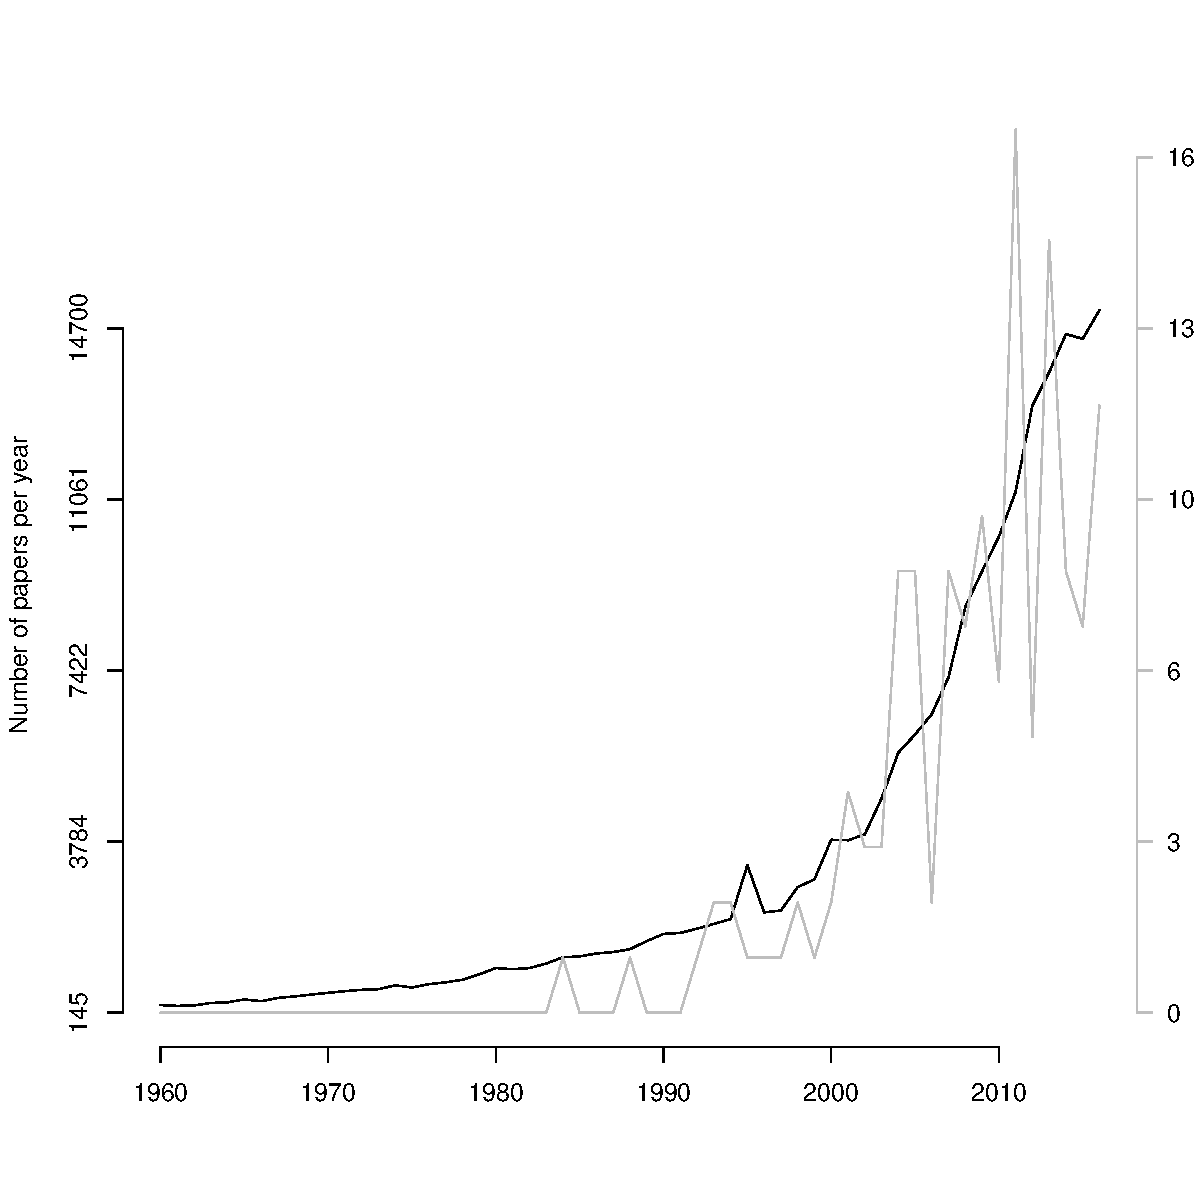
\includegraphics[width=1\textwidth]{Figures/GoogleScholarOccurences.pdf} 
% \caption{Number of papers on Google Scholar matching the search ``morphological disparity'' per year. In black, the match is in the paper and in grey, in the title. We collected the number of matches per year from 1960 to 2016 in Google Scholar for the terms "morphological disparity" both in the text (fuzzy matching) or in the title (exact matching). The data was collected on the 1st of November 2017.}
% \label{Fig:GoogleOccurences}
% \end{figure}


% \section{What actually \textit{is} disparity?}

% \cite{prentice2011} define disparity as: ``a term widely (albeit not always consistently) used to describe the range of forms in a group of organisms, or the difference among different body plans''.
% Disparity can describe either the metric (\citealt{Wills2001}; or index \citealt{Hopkins2017}) or the whole pipeline \citep{zelditch2012geometric,lloyd2016estimating}.
% To assess the usage of disparity in different published studies, we collected methodological data from the 500 first Google Scholar results for the key words ``morphological disparity'' per order of appearance (accessed on the 1st of November 2017).
% For the 230 relevant papers among the 500 matches, we collected the following methodological data: (1) What was the focal biological group? ; (2) What kind of data was measured (e.g. landmarks, discrete data, etc.)?  ; (3) Was data collected on the full organism or not? ; (4) How was the morphospace explicitly defined (e.g. PCA, PCO, MDS, etc.)? ; (5) How was the disparity metric(s) explicitly defined? ; (6) Which statistical test was applied to test the disparity related hypothesis? ; (7) Was phylogeny taken into account or not?
% We used only the explicit definition of the morphospace and the disparity metric(s) in this search since a few number of papers had a vague definition of either or both (e.g. a disparity metric was measured but not described anywhere in the paper).
% The remaining 270 matches were disparity was mentioned but not measured felt in the following categories: papers out of topic, papers mentioning morphological disparity without measuring it, review papers, papers not accessible (either through a broken link or a paywall) or referenced citation without the paper (as a Google Scholar match).
% To reduce the amount of categories for the 230 recorded methods, we concatenated different methods in a smaller number of categories (see supplementary materials and \url{https://github.com/TGuillerme/Disparity_Working_Group/blob/master/Analysis/data_cleaning.Rmd}).

% \begin{figure}[!htbp]
% \centering
%    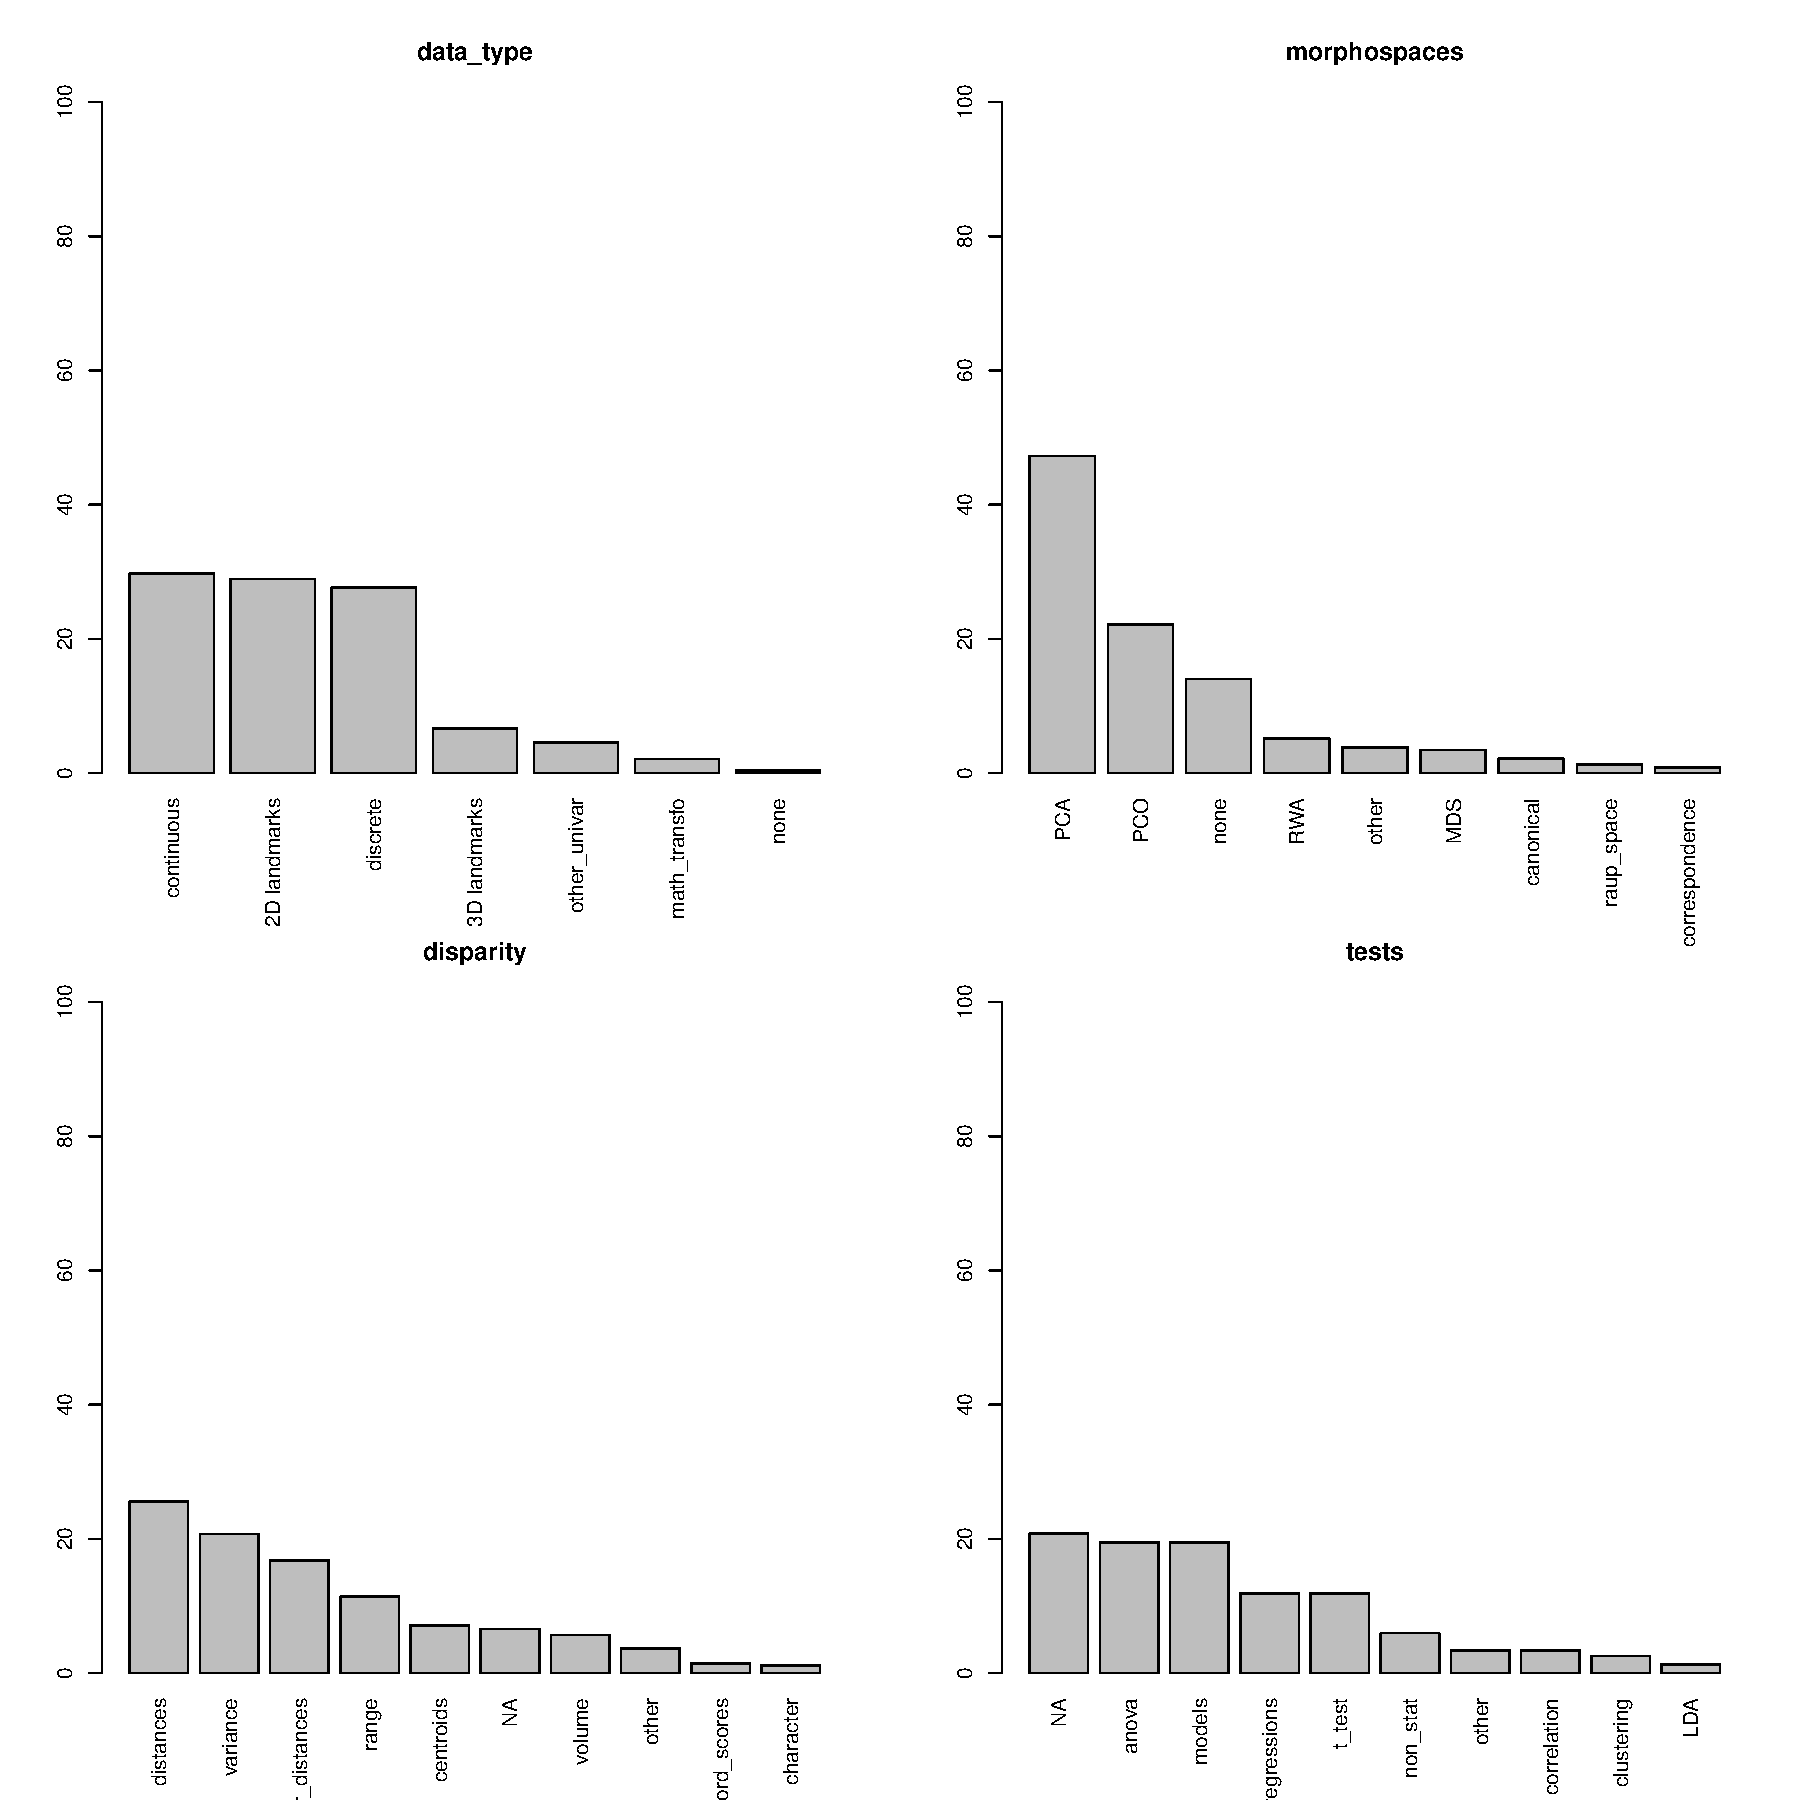
\includegraphics[width=1\textwidth]{Figures/MethodsProportions.pdf} 
% \caption{Disparity methods proportional usage: (1) Data type: which input data was used (...); (2) Morphospace: how was the morphospace obtained (...); (3) disparity: what type of disparity metric was calculated (...); (4) test: what type of test was applied (...).}
% \label{Fig:MethodsProportions}
% \end{figure}

% From the collected data, we can highlight the use of three main different disparity analysis with their associated data/morphospace/metric/tests and related to specific methodological implementations.

% \begin{itemize}
%     \item \textbf{The ``\texttt{Claddis}'' approach:} this group of methods uses discrete morphological data (sometimes referred to as ``Cladistic'' characters) for the full organisms to build a PCO from the organism's pairwise distance as a morphospace. Disparity is then often measured as a variation of the ordinated matrix dimensions' variances or ranges (e.g. the sum of variance or/and the sum of ranges). Hypothesis are often tested using multivariate ANOVAs on the pairwise distance matrix or by simply comparing the confidence intervals overlap of the disparity from different groups. 

%     \item \textbf{The ``\texttt{geomorph}'' approach:} this group of method is based on landmark data (2D or 3D) on parts of the organism studied usually the skull) and use a Procrustes transformation of the landmarks that are then directly ordinated using a PCA (but sometimes RWA). Disparity is often measured as a distance metric (e.g. the distance between the species and a point in the morphospace such as its centroid). Hypothesis are then tested using ANOVA type tests with usually no phylogenetic correction (although phylogeny is sometimes used to correct the morphospace).

%     \item \textbf{The ``\texttt{approach}'' approach:} this method can directly use continuous or discrete data for the full organism without any ordination (but not necessarily), and will measure disparity as the average pairwise distance between species (whether euclidean or any other type of distance). Hypothesis of higher/lower disparity can then be measured using null evolutionary models.
% \end{itemize}

% %
% The advent of these three approaches coincides with the explosion of disparity analysis (Fig. \ref{Fig:GoogleOccurences}) and suggest a high popularity of disparity analysis.
% %
% Unfortunately, however, few actual tests have been performed on whether any of these approaches \textit{actually} allows to tackle the classic disparity questions (see \ref{text:intro}{Introduction}).
% Are all these methods the right tools to answer these questions are they mere ``inductive fishing trips'' used to describe the data rather than testing any of the hypothesis related to the disparity questions?

% \section{Does data used in disparity analysis allows to test hypothesis?}
% In fact, the question of which data to analyse \citep{hetherington2015cladistic} and which part of the data to use has been analysed \citep{hopkins2017well} has rarely been assessed.
% Can the data used in disparity studies actually test the phenomenon researchers are trying to capture?

% For example, when studying discrete morphological characters (often following the ``\texttt{Claddis}'' approach), the data used is often recycled data used for phylogenetic analysis.
% These datasets are usually design to recover evolutionary history and differentiate clades and, often due to the preservations of the fossil record, are mainly based on hard tissue characters.
% In phylogenetics, this artefact have been shown to be leading to measurable topological recovery error (for soft \textit{vs} hard characters; \citealt{sansomfossilization2013}; or dental \textit{vs} cranial characters \citealt{sansom2017dental}).
% Therefore, is the morphospace composed of ``fossilisable'' characters enough for answering evolutionary hypothesis?
% For example, are niche replacement hypothesis equivalent to fossilisable-character-based-niches replacement hypothesis?

% Similarly, many studies in geometric morphometric are based solely on skull shape using landmark techniques combined with Procrustes superimposition \citep[the ``\texttt{geomorph}'' approach;][]{zelditch2012geometric,adams2017geometric}.
% However, it has been shown that the whole skeleton displays different integrated modules with different specific evolutionary constraints leading to variable rates and modes of evolution (\citealt{Goswami20130254}; and this even at the cranial level \citealt{goswami2010influence}).
% Is skull variation enough for measuring body plans variation through time for example?

% In the case where disparity is measured a single continuous trait (or a collection of traits; following the ``\texttt{geiger}'' approach), for example in \cite{price2014niche}, beak and limb length as well as body mass are used to differentiate groups of birds and different zones in the morphospace can then be interpreted as different niches.
% Is this set of traits studied in isolation sufficient to test niche occupancy hypothesis?

% Additionally, in many cases, the disparity metrics and hypothesis are often based on a transformation of the data (pairwise distances, PCA, PCO, MDS, RWA, etc.).
% Can these transformation readily reflect the raw data in our hypothesis?
% For examples a morphospace as a pairwise matrix reflects the dissimilarity between the data, a morphospace based on an ordination reflects the variability within the data, a morphospace based on both reflects the variability within the dissimilarity, are each method reflecting that?

% \section{Do the disparity metrics (or indices) really reflect variation in the studied phenomenon?}
% From the 230 papers analysed, we found 104 unique combination's of metrics to measure disparity (Fig. \ref{Fig:MethodsProportions}).
% Commonly, these metrics are used to approximate the volume occupancy within the morphospace \citep{Wills2001,DonohueDim,diaz2016global}.

% However, it has been shown that different metrics reacts differently depending on the dataset \citep[][; and an anecdotal example in Fig. \ref{Fig:DimensionsEffect}]{Wills2001,Ciampaglio2001}.
% For example metrics involving a product of aspects of the matrix (e.g. the volume, the product of the dimensions) are likely to suffer from the \textit{Curse of dimensionality} \citep{bellman1957dynamic} and will quickly tend to null values.
% Some other metrics are not representing all the data captured in the morphospace (e.g. the sum or product of variance ignores the co-variance between dimensions).
% Are these metrics as a description of the ordination a good proxy for the observed biological phenomenon?


% \begin{figure}[!htbp]
% \centering
%    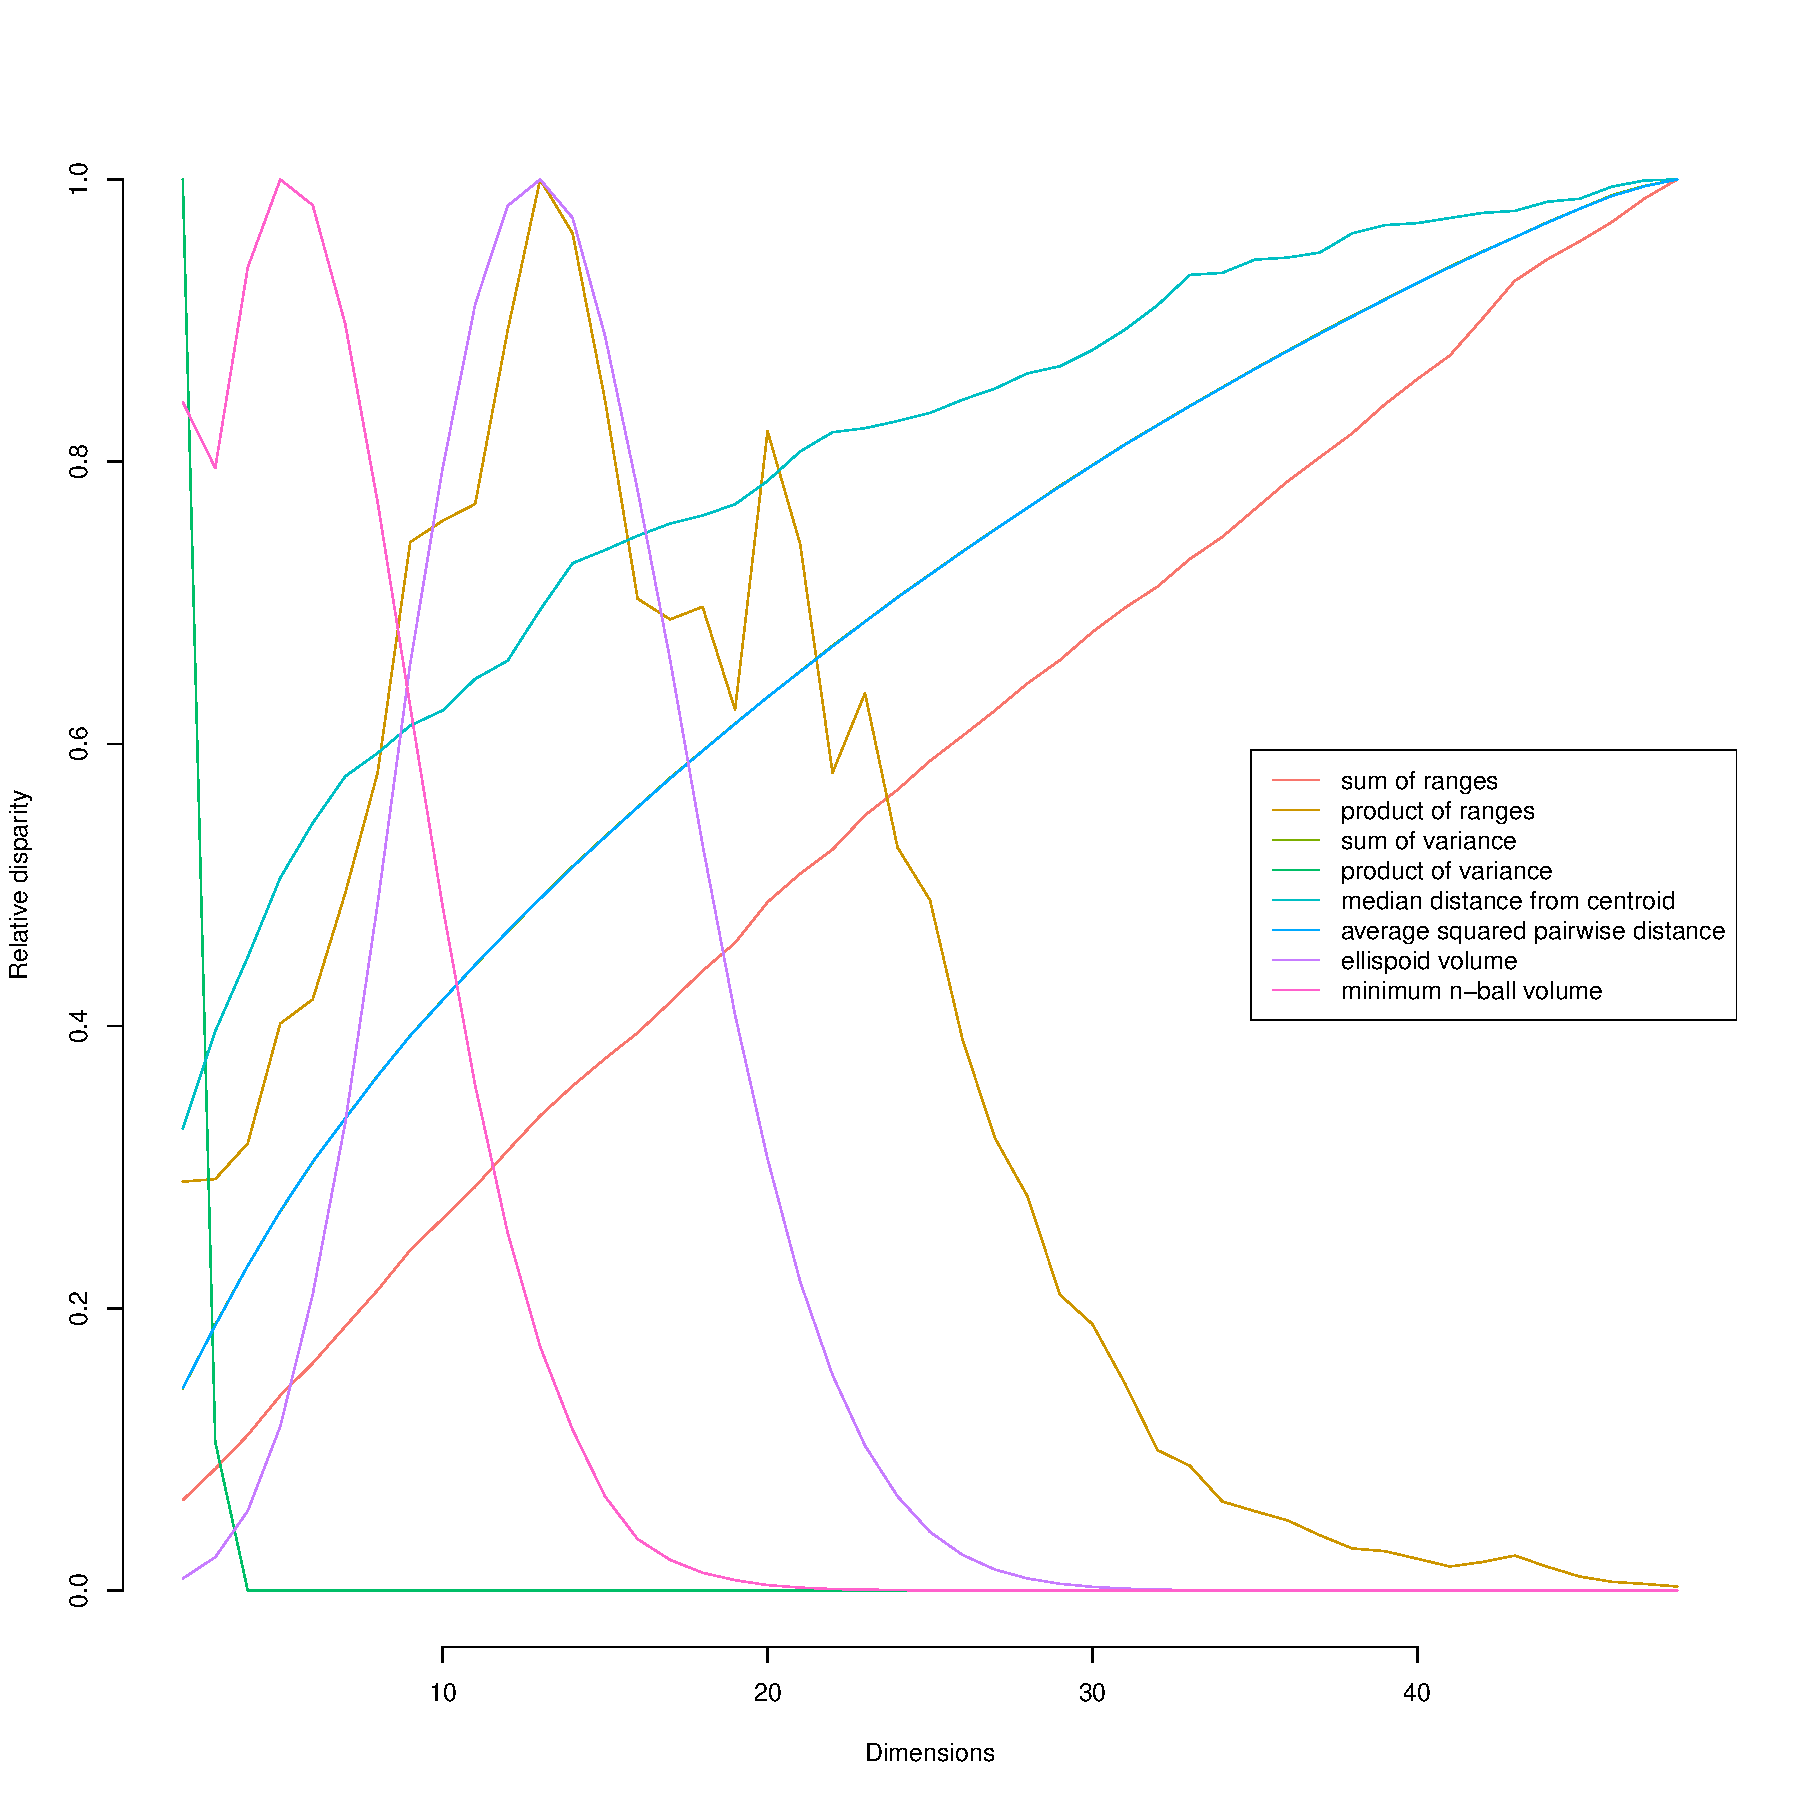
\includegraphics[width=1\textwidth]{Figures/DimensionsEffect.pdf} 
% \caption{Effect of the number of dimensions on different disparity metrics (note that the sum of variance is equal to the average squared pairwise distance in this case).
% The data used is one of the example datasets from the \texttt{dispRity R} package \citep[\texttt{BeckLee\_mat50};][]{beckancient2014,dispRityv02} composed of 50 elements and 48 dimensions obtained from a ordination (MDS) of the distance matrix of a discrete morphological character matrix.}
% \label{Fig:DimensionsEffect}
% \end{figure}

% Despite these caveats, it is important to actually know what the metrics are measuring.
% There has been some attempts to test that through simulations \citep{Ciampaglio2001,  gerber2017geometry} but it is still unclear which metric reflects the best the hypothesis test.
% For example, the average squared pairwise distance (or the sum of ranges) are really popular \citep[e.g.][]{geiger2008} yet has been shown to be fairly senstive, at least in empirical data to the number of sampled taxa, the number of characters and the data completeness \citep[][; although effects were lesser in simulations]{Ciampaglio2001}.
% More fundamentally, the question arises whether one disparity metric could be sufficient to describe changes in disparity?
% Changes in multidimensions might not be readily grasped by unidimensional metrics!
% For example, a given taxonomic group might have the exact same volume as another one yet be in a complete different part of the morphospace \citep[or even overlap or not depending on the dimensions;][]{davis2012acanthodes,brusatte50}.
% In this case, it might more interesting to have multiple metrics (e.g. the position and the volume) [FABRE et. al in prep.] or to use distributions of metrics (e.g. what does the average distance between species or from a point really convey? Is the distribution not more interesting?).

% Maybe we need metrics that fit explicitly our hypothesis (or fit our hypothesis directly to the metric).
% For example, for competitive replacement, should we not measure whether group A occupies the same place as group B through time and whether that is due to competition or simply because any other place in the space cannot be occupied (and why are such spaces unoccupied)?


% \section{Is the current statistical toolkit sufficient for testing disparity hypothesis?}
% Are the methods used to test hypothesis in disparity actually testing what we think they're testing (problem of multidimensional hypothesis)
% What does an anova or related variance based test real infirm/confirms regarding the disparity questions?
% How do we deal with bootstrapped data and pseudo-replications?
% Can we realistically use univariate Gaussian models to test hypothesis based on multivariate, probably non-Gaussian data? \citep{blomberg2017beyond}

% Should be take phylogeny into account? \citep{polly2013phylogenetic}



% \section{What are we missing?}

% \subsection{Learning lessons from other fields}
% In ecology, disparity bears strong parallels with $\beta$-diversity in ecology (a measure of ecological communities (dis)similarity): one biological observation described by a vast array of metrics \citep{baselga2010partitioning, anderson2011navigating, donohue2016navigating}.

% \section{Conclusion}
% We need a more hypothesis driven way of analysing disparity.
% Disparity methods should be the tool for answering disparity hypothesis, not merely a description of the data.




% \hl{[ADD Biological group, full organism and phylogeny in the supplementary]}

% \noindent \hl{\textit{These points should be developed during the meeting}}


% \subsection{Disparity data}
% The data used for disparity methods comes from three main sources:
% \begin{itemize}
%     \item Continuous data such as limb or body measurements \citep{slaterCetacean}.
%     \item Discrete morphological characters \citep[sometimes referred to as ``Cladistic'' characters; ][]{Brusatte12092008}.
%     \item Geometric morphometric data which is generally the Procrustes transformation of 2D or 3D landmarks \citep{cooney2017mega}.
% \end{itemize}

% However, data was by far not limited to these three categories (e.g. colours \citealt{maia2013key}; metabolic rate \citealt{nespolo2016studying} or chemicals signal \citealt{garcia2017heterogeneous}).

% \subsection{Morphospaces}
% \begin{itemize}
%     \item PCAs [CITE].
%     \item PCOs [CITE]
%     \item Pairwise distance matrices \citep[no ordination; ][]{Harmon961}.
% \end{itemize}

% But also RWA [CITE] or Raup-spaces [CITE].

% \subsection{Disparity metrics}
% Throughout the 230 analysed papers, we found 103 unique combinations of metrics!

% \begin{itemize}
%     \item Distances measurements between species or from a certain point in the morphospace [CITE].
%     \item Ranges and variances of each axis of the morphospace \cite{Wills2001,Ciampaglio2001}
%     \item Distance between species based on the pairwise distance matrix (not the ordinations) [CITE].
% \end{itemize}

% But also metrics based on the volume [CITE], the characters dissimilarity [CITE] or the coordinates of some axis of the ordination [CITE]

% \subsection{Disparity hypothesis}
% Describing the many outputs (what and how is it tested):

% \begin{itemize}
%     \item Variance based (ANOVA, etc.) [CITE].
%     \item Correlation based [CITE].
%     \item Regression based (PGLS, etc.) [CITE].
% \end{itemize}

% But also discriminant analysis [CITE] and clustering [CITE].

% Of course some studies use a combination of these three methods or none of them at all!

% Also, among each category XX\% of studies use multiple approaches.

% [ADD Biological group, full organism and phylogeny in the supplementary]

% \section{Expanding disparity}

% How to compare disparity between groups? Is disparity relative?

% How to compare disparity between methods?

% Can we really say things about competition when looking at disparity in a single group?

% Are all characters equal? Character contingency suggests otherwise

% What is the relationship between disparity and tree shape?

% Do we have a null model for investigating disparity?

% Can we really say things about competition when looking at disparity in a single group?


% \noindent \hl{\textit{Disparity in other fields}}

% In ecology, disparity bears strong parallels with $\beta$-diversity in ecology (a measure of ecological communities (dis)similarity): one biological observation described by a vast array of metrics \citep{baselga2010partitioning, anderson2011navigating, donohue2016navigating}.

% \section{Conclusion}

% A quick guideline for good disparity analysis:

% Maybe we need something like in Parham et al 2012 (Best Practices for Justifying Fossil Calibrations): an easy an identifiable description of the pipeline containing: 1) the type of data, 2) the morphospace and 3) the metric? 

\section{Authors contribution}
TG, NC and PD proposed the idea of this review. TG, NC, SB, KD, AJ, SG, AG, KH, MH, GL, JOR, AP, ER, ES, ES, GS, GHT and PD wrote the manuscript,

\section{Acknowledgments}
The Royal Society.
TG acknowledge support from European Research Council under the European Union's Seventh Framework Programme (FP/2007 – 2013)/ERC Grant Agreement number 311092 awarded to Martin D. Brazeau.


\bibliographystyle{sysbio}
\bibliography{References}

\end{document}

